\documentclass[tikz, border=0.5cm]{standalone}
\usetikzlibrary{shapes}
\usetikzlibrary{positioning}
\begin{document}
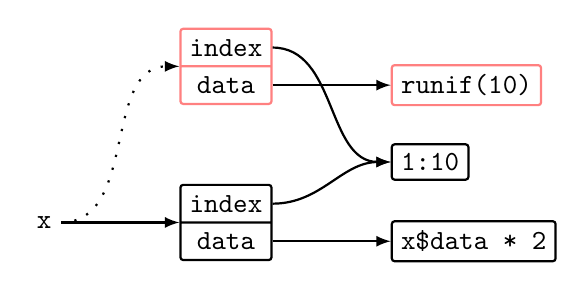
\begin{tikzpicture}
\node[
  thick,
  draw=red!50, rounded corners=1pt,
  rectangle split,
  rectangle split parts=2, 
  rectangle split draw splits=true] (df1) {\texttt{index}\nodepart{two}\texttt{data}};
\node[
  thick,
  draw, rounded corners=1pt,
  rectangle split,
  rectangle split parts=2, 
  rectangle split draw splits=true,
  below=1cm of df1] (df2) {\texttt{index}\nodepart{two}\texttt{data}};
\node[left=1.5cm of df2] (x) {\texttt{x}};
\node[
  thick,
  draw=red!50, rounded corners=1pt,
  right=1.5cm of df1.two east] (data1) {\texttt{runif(10)}};
\node[
  thick,
  draw, rounded corners=1pt,
  right=1.5cm of df2.two east] (data2) {\texttt{x\$data * 2}};
\node[
  thick,
  draw, rounded corners=1pt,
  above=0.5cm of data2.north west,
  anchor=south west] (index) {\texttt{1:10}};
\draw[-latex, loosely dotted, thick] (x.east) to[out=0, in=180] (df1.west);
\draw[-latex, thick] (x.east) to[out=0, in=180] (df2.west);
\draw[-latex, thick] (df1.text east) to[out=0, in=180] (index.west);
\draw[-latex, thick] (df2.text east) to[out=0, in=180] (index.west);
\draw[-latex, thick] (df1.two east) -- (data1.west);
\draw[-latex, thick] (df2.two east) -- (data2.west);
\end{tikzpicture}
\end{document}
